Esta seção tem como objetivo mostrar aplicação do paralelismo sobre os
algoritmos analisados neste trabalho.

\subsection{OpenMP}

Para a aplicação do paralelismo utilizando a biblioteca OpenMP, foi utilizada a
abordagem de processar uma imagem por vez, mas subdividindo as imagens em quatro
partes iguais. Um exemplo dessa subdivisão pode ser vista na
Figura~\ref{fig:lena}.

\begin{figure}[!h]
	\centering
	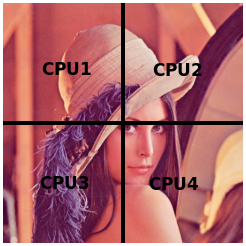
\includegraphics[width=0.3\linewidth]{figs/lenna.png}
	\caption{Subdivisão das imagens.}
	\label{fig:lena}
\end{figure}

Cada processador fica responsável por realizar o algoritmo de conversão em
escala de cinza em uma determinada região da imagem (quando é utilizado
realmente 4 \textit{threads}). Todo esse processo é realizado para cada imagem
até que todas as imagens sejam processadas.

\subsection{OpenMPI}

Já para a aplicação do paralelismo utilizando a biblioteca OpenMPI, foi
realizada a abordagem de processar uma imagem em cada núcleo de processamento.
Dessa forma, blocos de no máximo quatro imagens são carregados de uma vez para o
processamento. A Figura~\ref{fig:mpi} ilustra a aplicação dessa abordagem.

\begin{figure}[!h]
	\centering
	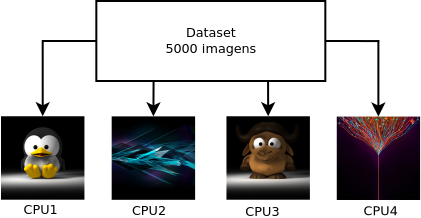
\includegraphics[width=0.5\linewidth]{figs/mpi}
	\caption{Abordagem aplicada.}
	\label{fig:mpi}
\end{figure}

A quantidade de imagens carregadas é igual a quantidade de núcleos de
processamento utilizado. A imagem~\ref{fig:mpi} mostra o carregamento de quatro
imagens de uma vez para ser processadas por quatro núcleos de forma
independente. Esse tipo de abordagem causa um desbalanceamento quando é
executado com três núcles, pois a quantidade de imagens da base não é divisível
por três.




